\documentclass[a4paper,12pt]{report}
% document customization
\usepackage[margin=1in]{geometry}
% load custom font
\usepackage{fontspec}
\setmainfont{Carlito}
% code/monospace
\usepackage{listings}
\lstset{
	postbreak=\mbox{\textcolor{red}{$\hookrightarrow$}\space},
	basicstyle=\small,
}
% ability to use \FloatBarrier
\usepackage{placeins}
\usepackage{graphicx}
\usepackage{tabularx}
\graphicspath{{./assets/}}
\usepackage{wrapfig}
% pdf
\usepackage{pdfpages}
% charts
\usepackage{bchart}
% href links
\usepackage[hidelinks]{hyperref}
\hypersetup{
    colorlinks,
    allcolors=black
}
% glossaries
% add 'nomain' if no main glossary exists
\usepackage[nomain,acronym,nopostdot]{glossaries}
\newacronym{udp}{UDP}{User Datagram Protocol}
\newacronym{tcp}{TCP}{Transmission Control Protocol}
\newacronym{sctp}{SCTP}{Stream Control Transmission Protocol}

\makeglossaries
% remove glossary section titles
\renewcommand{\glossarysection}[2][]{}
\usepackage{bookmark}
% create bibliography
% run 'biber <tex name>' to convert .bib files
\usepackage[style=authoryear-ibid,backend=biber,natbib=true]{biblatex}
\addbibresource{refs.bib}
\addbibresource{web-refs.bib}
% section customization
\usepackage{titlesec}
\titleformat{\chapter}{\normalfont\huge}{\thechapter.}{20pt}{\huge\it}
\titlespacing*{\chapter}{0pt}{-60pt}{20pt}
% caption customization
\usepackage[labelfont=bf, skip=5pt, font=small]{caption}
% paragraph customization
\renewcommand{\baselinestretch}{1.25}
\setlength{\parskip}{1em}
\setlength{\parindent}{0em}


\begin{document}

\begin{titlepage}
    \rightline{\textbf{FAO} Allan Callaghan}

	\begin{center}
		\textbf{School of Engineering, Technology and Design}

		\textbf{BSc (Hons.) Computer Science}

		\textbf{2022-2023}

		\textbf{IP 40}

		\vspace{4ex}

		\textbf{Title:}

		Engineering Investigation Into File Synchronisation Protocols

        \textbf{Author:} Leo Spratt

        \textbf{Supervisor:} Allan Callaghan

        \textbf{E-mail:} ls959@canterbury.ac.uk

		\vspace{4ex}

        \small{This report is submitted in partial fulfilment of the requirement for the BSc in \textsl{Computer Science} at Canterbury Christ Church University

		I declare that this report is my own original work containing no personal data as defined in the Data Protection Act (1998) and that I have read, understood and accept the University's regulations on plagiarism/intellectual property rights/research ethics (in particular the Research Governance Handbook) and the IP 40 Module Handbook.

        Finally, I accept that no copy of my Individual Project 40 will ever be returned regardless of the circumstances.}

		Signed: \verb|              |

		Date Of Submission: 5th May 2023
	\end{center}
\end{titlepage}

% \nocite{*} % add any unsighted references to bibliography

\begin{abstract}
	This report investigates into the domain of file synchronisation at the network level. Exploring whether a modern solution can be built to utilise modern technologies and out perform existing solutions. Prototypes are built and compared against the existing solutions (FTP, SMB and rsync) to achieve this, measuring total network overhead and performance via maximum transfer speed. The findings shown from testing shows that a newer solution could improve in the future by using methodologies such as building on top of UDP and implementing dynamic error correction. Although testing showed that more overhead was sent, transfer speed was dramatically increased compared to the existing solutions proving that networks can be better utilised using modern tooling.

\end{abstract}
\chapter*{Acknowledgements}
Allan Callaghan who was my project supervisor, for all his support and enthusiasm for my project.

My parents who have always supported me throughout my education.

My first Computer Science teacher Lance Jacobs, who inspired and encouraged me to expand my programming knowledge further.

\tableofcontents
\newpage
\listoffigures
\newpage
\listoftables
\newpage
\lstlistoflistings
\newpage
\chapter{Introduction}
A lot as changed since the TCP/IP stack was put into use. We now rely heavily on computers to aid us in everyday life. An extreme amount of data is transferred across large networks powering the "cloud" that allows people to use powerful software on their many devices.

However with the greater demand and improvements to technologies there has been little improvement to existing lower level technologies such as protocols. As the world creates more data, most people do not want to lose it, so it is backed up using well established (and old) protocols such as the FTP family, SMB and rsync that are all based on the TCP protocol.

A modern solution could be very beneficial to be more efficient and fully utilise modern technologies that are available, while removing compatibility for archaic devices which could potently hinder any improvement.

\chapter{Legal Considerations}
There are no legal considerations.
\chapter{Ethical Considerations}
There are no ethical considerations.
% START main chapters
\chapter{Existing Solutions}
\section{Solutions To Investigate}
To compare the prototypes against, a range of existing solutions need to be first investigated and tested to allow a more accurate comparison.

There are many solutions that have been created to transfer files. Listed below are the solutions that will be compared:

\begin{itemize}
	\item SMB2
    \item FTP
	\item rsync
	\item SyncThing
\end{itemize}


\section{How They Work}
\section{Testing}
\section{Comparison}

\chapter{Research}
\section{The Transport Layer}
Currently as of 2023 networked devices use the TCP/IP stack. This includes the TCP and UDP protocol.

\subsection*{UDP}
UDP is the oldest protocol at the transport layer. It is also the least complex, since it features only necessary parts to allow transmission of packets across networks. It is a connectionless protocol, meaning it has no handshake to establish a new connection and has no form of reliability or other error handling \parencite{udp-rfc768}.

This would make UDP on it's own is unsuitable for any reliable communication on it's own. Early use-cases were for real-time video/audio streaming and games.

This would seem to make UDP unsuitable for any reliable communication. However since protocols can be built on top of UDP to implement reliability and other features specifically targeted for the task, in recent years it has seen more use for forming the basis of reliable data transfer.

For example a modern protocol that has widespread use today is QUIC. It is built on top of UDP, providing all the necessary reliability features in the application layer. It is designed to have improved performance over TCP. Currently it is most used for serving website content over http/3 which uses QUIC.

UDP is also used in VPN protocols such as WireGuard and OpenVPN. These also have reliability built-in allowing for low latency access of remote networks.

Using UDP for reliable applications is possible since most networks have limited packet loss, due to more modern network technology being used such as switches; eliminating packet collisions.

It is now common for newer protocols to be built using UDP since it is wasteful having TCP acknowledgements for every packet since it increases the latency, due to the constant pausing for acknowledgements.

Despite UDP having no form of error correction, it does have a single checksum field in the header. Depending on the situation it can even be disabled. This checksum is usually only validates the headers are not corrupted leaving the payload to possibly have been corrupted. An under-used part of the specification is to enable the checksum to include the payload as well, meaning that the whole packet could be validated and ignored if corruption occurred.

Using the checksum field for payload validation allows for corruption to be detected directly via hardware such as the NIC instead of implementing a application level one. This would allow a packet to be discarded before it even reaches the app. Removing the need to check for corruption at the application layer reduces the amount of possible scenarios to handle. Most UDP applications that need to be reliable would need to handle packet loss, reordering and duplication.

For UDP to have the same reliability as TCP, it could be reimplemented to match TCP, however that would not improve over what already exists, as TCP could just of been used. Instead a custom solution built specifically for the task could be built. As mentioned before most internal networks now have limited packet loss, meaning that selective error checking could be implemented, allowing for a lower latency and higher throughput transfer.

\subsection*{TCP}
Building from UDP; TCP is the most commonly used protocol. Providing many features such as detection of lost packets and handling of out of order packets. All of this can be implemented and processed at the kernel level, reducing the need for a developer to implement it in their application \parencite{tcp-rfc793}.

This in-built reliability would of been important at the time most of these protocols were created, since machines at that time were limited on the amount of processing power and memory available. The reliability of TCP would have been important as many networks would have been using network configurations such as a BUS or RING to link computers together which were renowned for having packet loss due to packet collisions.

TCP is still the most used protocol because of the in-built features, meaning that developers of programs do not need to worry about implementing their own error checking. Because of the widespread use it also guaranties device support, meaning greater compatibility.

\subsection*{SCTP}
There are many modern protocols being developed, one of these is SCTP (Stream Control Transmission Protocol). This protocols goal is to improve on the TCP and UDP drawbacks. Offering reliable in-order data transfer while having a simpler packet structure compared to TCP, having two main sections; the header and chunks. There can be multiple chunks per packet with two different types available, payload data and control messages, this allows for smaller messages to be bundled together if they can fit inside one packet; thus reducing network overhead. SCTP keeps a connection open by using "heartbeat" messages, this ensures both ends of a connection knows whether they can still access each other \parencite{sctp-rfc9260} \parencite{ladha2004improving}.

SCTP seems like a suitable improvement over TCP and UDP, however it has drawbacks. Mainly it's limited adoption which is most likely due to the RFC still being in a "Proposal" stage. This is a problem since it is a transmission protocol, it requires all receiving devices on the network to understand it; this would include routers and switches. This limited adoption would therefore cause issues as you would have to ensure that all devices supported it, otherwise packets may be detected as unknown and dropped by the unsupported devices; due to packets being treated as corrupted or malicious.

This limited supports means that it is currently unsuited for use, until more devices have support and the protocol is fully standardised and can then be supported by more network devices.

\subsection*{Conclusion}
It seems like the suitable way of implementing an improved file synchronisation/transfer protocol is by using UDP and building custom reliability features specific for the application; in the application layer. There will be many ways that the reliability could be implemented and these will be investigated during prototyping.


\section{Data Format}
Before experimental prototypes can be made, investigating how to structure the data which will be contained in the packets payload should be investigated.

\subsection*{Telnet Strings}
Using plain ASCII text for messages; would allow the protocol to work on archaic devices. However modern devices are being targeted, making this format unsuitable since it would increase the amount of network overhead required for sending ASCII messages. It would also not have a way of easily representing structured data.

\subsection*{JSON}
JSON is the most common format seen in web based technologies, however it would be unsuitable for a protocol; since it requires all data to be encoded as ASCII so any binary data would have to be encoded for example using base64. This extra encoding step would increase both complexity and the required processing power needed to handle each packet \parencite{json-rfc8259}.

\subsection*{MessagePack}
MessagePack (or CBOR) is also another format that could be used, it is more suitable for a protocol since it is encoded directly into binary, also removing the need to encode binary data as this data can be stored directly as a bytes type. However like JSON it is also schema-less. So extra validation would have to occur when checking validity of a message \parencite{msgpack} \parencite{cbor-rfc8949}.

\subsection*{Protocol Buffers}
A newer format is protobuf. This format is designed specifically for serializing structured data using pre-defined schemas, meaning validation of a message can be checked easily, since the expected format is known from the created schemas. Having a required schema makes it more suitable for use in protocols which have a pre-defined structure. Like MessagePack it is also a "binary wire" format making the serialized result as small as possible \parencite{protobuf-3}.

\subsection*{Conclusion}
After investing possible ways of formatting data to send as a payload for network packets. Protocol Buffers seem suitable for this project, as they require schemas to be defined and do not require extra serialization steps when sending binary data.

\chapter{Prototyping}
As this project is purely an investigation into whether a more modern solution for transferring files can be produced, these prototypes will only focus on the minimum possible required to have functionality. This allows for each prototype to improve on the most important features. These are listed below:

\begin{itemize}
	\item Error correction
	\item Sending files from client to server
	\item Adjustable settings, for testing
	\item Only support a single client connection
\end{itemize}

To test the prototypes, the previous methodology of testing will be used. This is documented in Appendix~\ref{sec:testing-environment}. On the virtualised network, these prototypes will use the maximum available MTU size which is 65,000 bytes which matches the previous tests.

\newpage
\section{Prototype One}
\subsection*{Solution Design}
The first prototype will take inspiration from FTP streaming for file data transfer. Using UDP with this should reduce the total latency for a transfer; since all file data packets can be sent with no interruption for waiting for acknowledgments.

This prototype will use the binary protobuf format for structuring the packet data. This will reduce the amount of required overhead needed for storing structured data. Binary is suited for this prototype since it does not need to be easily human readable since only the software will be directly interacting with the data.

\subsubsection*{Packet Structure}
The packets structure will be split into several fields, using flexible offsets meaning the packet size is dynamic. Having a dynamic packet size should reduce the amount of wasted space, leaving more available space for the actual file data.

A packet will feature two protobuf fields one for the header which will describe what the packet is, and the second will include any extra metadata relevant to a request/response. The packets fields are illustrated in Table~\ref{tab:p1d-packet-fields}.

\begin{table}[h!]
    \caption{Prototype One Packet Fields}
    \label{tab:p1d-packet-fields}
    \centering
    \begin{tabular}{ l l l }
        \hline
        \textbf{Num} & \textbf{Name}   & \textbf{Data-Type} \\
        \hline
        001          & Type            & uint8              \\
        \hline
        002          & Header Length   & uint64             \\
        \hline
        003          & Header          & protobuf           \\
        \hline
        004          & Metadata Length & uint64             \\
        \hline
        005          & Metadata        & protobuf           \\
        \hline
        006          & Payload Length  & uint64             \\
        \hline
        007          & Payload         & binary             \\
        \hline
    \end{tabular}
\end{table}

The first field will take up exactly 1 byte, this field will be used to set the type of the packet. This will determine what protobuf encoded header structure will be. Using 1 byte will allow for 255 possible message types. Since these prototypes will not be a fully implemented solution only a few types will be implemented, which are shown in Table~\ref{tab:p1d-packet-types}.

\begin{table}[h!]
    \caption{Prototype One Packet Types}
    \label{tab:p1d-packet-types}
    \centering
    \begin{tabular}{ l l l }
        \hline
        \textbf{Prefix} & \textbf{Value} & \textbf{Note}                \\
        \hline
        SYN             & 1              & Perform connection handshake \\
        \hline
        ACK             & 2              & Acknowledge request          \\
        \hline
        REQ             & 3              & Request to send/receive      \\
        \hline
        PSH             & 4              & Send payload data            \\
        \hline
        FIN             & 254            & End connection               \\
        \hline
    \end{tabular}
\end{table}

The next field will take up 8 bytes, this will be big-endian ordered number which will say how many bytes of data to expect after for the header (an offset value).

After header length the actual header will follow, if there is no header the next field will immediately follow.

The 4th field will be the metadata length which is the same as the header length, however specifies the length of the metadata field.

The metadata field is the same as the header.

An example of a SYN packet in both a structured view and a hex representation of the binary data is shown in Listing~\ref{lst:p1d-example-structure} and Listing~\ref{lst:p1d-example-binary}.

\begin{minipage}{\textwidth}
    \begin{lstlisting}[caption={Prototype One Example Packet Structure},label=lst:p1d-example-structure]
|-------------------|
| 1                 | <- Packet Type
| 5                 | <- Header Length
| {id: 1, mtu: 470} | <- Protobuf Header (JSON representation)
| 0                 | <- No Metadata
| 0                 | <- No Payload
|-------------------|
\end{lstlisting}

    \begin{lstlisting}[caption={Prototype One Example Packet Binary},label=lst:p1d-example-binary]
 1 0 0 0 0 0 0 0 5 8 1 16 214 3 0 0 0 0 0 0 0 0 0 0 0 0 0 0 0 0
 ^ ^^^^^^^^^^^^^^^ ^^^^^^^^^^^^ ^^^^^^^^^^^^^^^ ^^^^^^^^^^^^^^^
 |        |             |              |               |
Type    Header        Header        Metadata        Payload
        Length                       Length         Length
\end{lstlisting}
\end{minipage}

\subsubsection*{Operation}
For a client to first connect to the server a simple handshake will occur. This has been based on the rsync protocol handshake which only requires one exchange at the start. The client will first send a packet type called "SYN" which includes the clients max receiving MTU size, this allows for the message size to be adjusted depending on the network structure. After the server has received it will acknowledge the handshake and send back it's own "SYN" packet, which will contain it's maximum supported receiving MTU and a generated client ID. This client ID will be stored at the server until the client disconnects, this will allow for a connection to remain available without the client needing to renegotiate. Because this ID will be used to determine which client is which, each message sent by the client will need this ID attached. Every message from the client following "SYN", must also increment a request ID field, which will allow error checking functionality.

Since UDP is used error handling for missing and out-of-order packets is needed and for the server to know when the client has received the response from the server. This is already a implemented feature in TCP, so this prototype will be based off how TCP works. Each request message sent from the client will expect a "ACK" packet which will contain the request ID in the header, so the client can handle out-of-order and missing messages. There will a timeout duration for waiting for a "ACK", after the timeout the original message will be sent again. This will repeat until a "ACK" is received.

After a handshake, the client is free to send a request which in this prototype; will either be a request to send a file or ending the connection.

To request to send a file; a packet type of "REQ" is sent with the destination file path and file size in the packets metadata field, including the size allows the server to decide whether there is enough space to receive the file and reserve it. The server will reply with an "ACK" and the client will send the file data in a streaming fashion, each packet will be a "PSH" type containing the chunk ID and the request ID. A chunk ID is needed to reconstruct the received data at the server side so it is in the correct order, this ID is simply a incrementing number. The "PSH" packets will not have "ACK" responses from the server, instead validation will happen after the transfer. This has been designed to reduce the latency during a transfer since most networks have little to no packet loss.

Once a transfer is finished the client will send a "REQ" packet containing the last chunk ID. The client will then either receive a "ACK" from the server if no chunks are missing, or a "REQ" packet containing the missing chunks; causing the client to send "PSH" packets containing the missing chunks. This will repeat until a "ACK" is received.

To end a connection, the client will send a "FIN" packet, this will include just the client ID. The server will recognise the request to end and clear the client ID and "ACK" the request.

A sequence diagram example of a complete transfer is shown in Figure~\ref{fig:p1-sequence}.

\begin{figure}[h!]
    \centering
    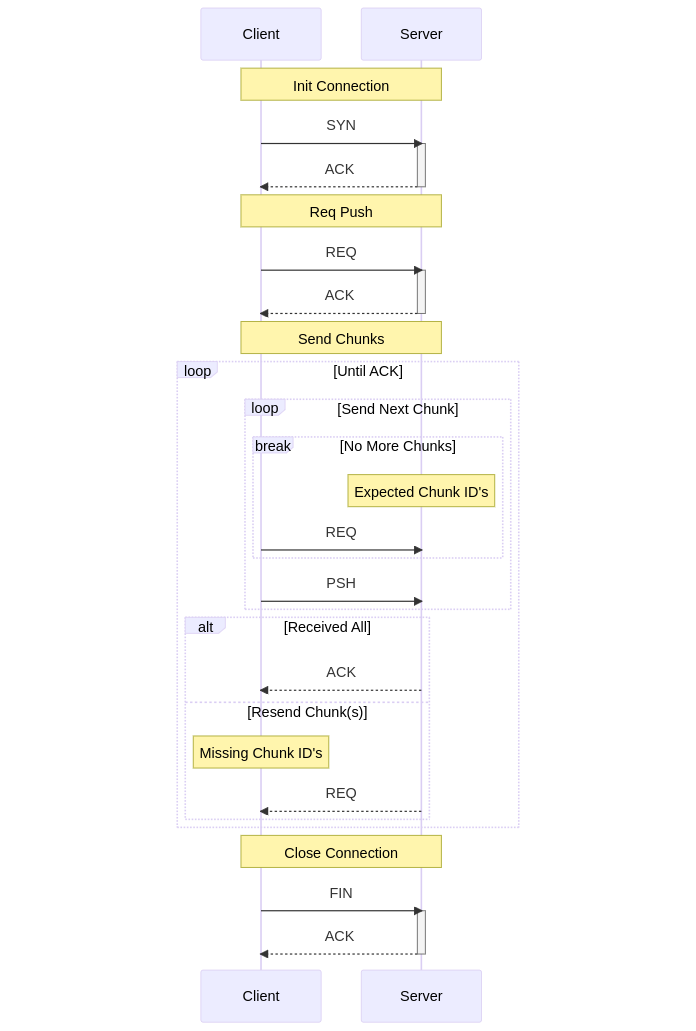
\includegraphics[width=0.8\linewidth]{p1-sequence.png}
    \caption{Prototype One Sequence Diagram}
    \label{fig:p1-sequence}
\end{figure}

\subsection*{Testing}
After the initial tests several issues in the code needed to be fixed. These are listed below (with git commit hashes):

\begin{itemize}
    \item (1e67ab) payload offset out by 1, causing payload to be incorrectly stored
    \item (dfb553) message size prediction code miss-calculates header + meta length fields, causing header and meta fields sizes to be incorrect; creating an invalid packet
    \item (35db84) client starting chunk id is 0, should be 1
    \item (455708) buffer payload was not copied (instead referenced), causing next request to alter payload values
\end{itemize}

After testing prototype one it has been found that the overhead in transferring a single file is less than the existing protocols having only "0.14\%" overhead; shown in Table~\ref{tab:prototypes-test-results}. It also sent out less packets than the existing solutions, only "39".

When testing with text files the prototype produced "7.48\%" of overhead, comparing this to the best performing existing protocol rsync which was less "5.64\%". Whilst rsync is less it is only a
"1.84\%" more, this could likely be reduced further in a future prototype.

In the next test with a collection of photos; the prototype produced a higher overhead compared to all investigated existing solutions "1.73\%", however the number of packets sent is lower "1,128". This likely points to the individual packets for transferring the physical file data having more overhead. If this was the final solution, it would be ineffective for transferring larger files since the amount of wasted data would scale with the file size.

In the last test which used a purely synthetic scenario; sending many small files sized at 1KB. The prototype produced a overhead of "~18\%" extra compared to rsync which was the best performing existing solution. Compared to the photos test, this scenario shows that this prototype has a greater amount of overhead sent for negotiating a file before transfer. However this overhead may be acceptable as rsync provides little safeguarding around file locking, compared to this prototype which if fully completed would issue an error packet before allowing a transfer to occur. Compared to the other protocols which do implement file locks (FTP and SMB2); this prototype has a smaller overhead. Looking at the number of packets sent; shows that "2,504" were sent, comparing this to rsync only "69" were sent. This is a very large difference. This prototype can only send chunks relating to the current file until the next is negotiated, whereas in rsync multiple files can be included in a single packet, making it more suitable for transferring small files, when many can fit in a single packet. Reducing the number of packets sent over the network can reduce both latency and the amount of traffic transferred allowing the bandwidth to be repurposed for another task.

This test measured a "8.0Gbps" in transfer speed. Whilst that may seem very high it is due to UDP (and the prototype) not requiring acknowledgements for each packet.

During testing it has been discovered that when many file chunks during a large transfer are lost, it will only be until the end of the transfer before they can be re-sent. This is not ideal, since on a higher latency network it could be quite a long time before the end of a transfer; resulting in a longer total transfer time. This could be improved by sending the chunks in blocks, for example 20 chunk packets could be sent then verified until either missing ones are re-sent or a new block is started. This would allow for a smaller amount of chunks to be required to be re-sent during a large transfer.

It has also been found that having two serialized fields (header, metadata) is also not ideal, since multiple complex steps have to be taken until the message can be handled. First the packet type has to be inspected, then the header must be deserialized before the metadata can be processed. This could be reduced to where only a packet type and header is sent, this would also reduce the amount of reserved space in a packet for the metadata length field; which takes up 8 bytes.

\newpage
\section{Prototype Two}
\subsection*{Solution Design}
The second prototype will focus on improving the method of sending the chunked data. This is necessary improvement, as in the event of many packets being dropped during a transfer; it will not be until the end of the transfer until the lost packets can be recovered.

To solve this without sending and waiting for acknowledgments for each packet (re-implementing TCP) a different method must be implemented. On smaller transfers the number of lost packets to recover from will be less than a larger transfer, grouping several chunks into a block of chunks then verifying each block will likely solve this issue. A sequence diagram example of a complete transfer is shown in Figure~\ref{fig:p2-sequence}.

In prototype one during the end of a transfer only three request types were sent: request to send a file, the file data and a verify packet to check if any chunks were needed to be resent. In this prototype a new request type has been added for marking the end-of-file (EOF) and ending the file transfer. The request for verification will not end the transfer; instead it is repurposed for checking for missing chunks for the current group. This will reduce the complexity of needing the server to keep a record of the blocks.

The existing protocol packet fields from prototype (headers and metadata) will stay the same. Both the client and server code will need to be altered to handle the new request type and at the client side keeping track of how many chunks are sent per block will need to be implemented. Figure~\ref{lst:p2d-offset-variables} shows the variables required for calculating blocks

\begin{lstlisting}[caption={Prototype Two Offset Variables},label=lst:p2d-offset-variables,breaklines,numbers=left,language=go]
var lastChunkID uint64 = 0
var seekOffset int = 0

chunkIDToOffset := make(map[uint64]int)

eof := false
missingChunks := make([]uint64, 0)
\end{lstlisting}


\subsection*{Testing}
After running the first test; an issue in the code discovered and had to be fixed. This is listed below (with git commit hashes):

\begin{itemize}
    \item (cae32ef) file reader cursor position not set back after a requested resend, causing incorrect data to be sent on next PSH. Fixed by seeking to stored seek offset before reading
\end{itemize}

In the first test sending a single file resulted in a higher overhead than the previous prototype, it also now has a higher overhead compared to all the tested existing solutions now showing "6.24\%". This means that implementing the transfer in blocks increased the overhead due to more packets being sent, which is shown in the results Table~\ref{tab:prototypes-test-results} going from "39" packets to "45".

In the text and photos tests prototype two still performed better than FTP and SMB2, however worse than rsync and the first prototype having "2.44\%" more overhead when transferring text and "0.19\%" more when transferring photos. This shows that the extra overhead created for handling validation of each block creates more impact on smaller files. Looking at the synthetic 1KB files test, shows the overhead to be "6.54\%" greater than prototype one. This indicates the same issue found in the text and photos test results.

In this prototype, test transfer speeds have reduced from prototype one, for example in the photos test it went from "1.9Gbps" down to "255.9Mbps", whilst slower than rsync's 1.0Gbps it reached a much greater speed than both FTP and SMB2. It likely that the extra validation added can be optimised at the software side in the last prototype.

Adding the extra message to mark a file as EOF (end-of-file), has been proved to create more overhead when sending many files. However this extra feature should allow for longer transfers to handle missing data sooner; rather than waiting until the end. The next prototype will need to ensure packet size is kept to a minimum, to reduce this overhead.

During testing an issue was discovered during transfers with multiple blocks, when they arrive out-of-order. This issue causes the chunks for different blocks to be captured incorrectly causing a corrupted file. To handle this prototype three will need to allow the receiver of a transfer to see which current chunk relates to what block. This will however increase the size of each chunk packet, but is a necessary increase in overhead for vital error checking.

Allowing the server to also know the maximum number of chunks per block could also allow memory to be pre-allocated allowing for less time to be taken allocating memory and potentially reducing the number of dropped packets during a transfer on a lower spec machine.

Due to the seen higher overhead created in both prototype one and two, the field sizes need to be reduced. Reserving 8 bytes each for the header, metadata and payload lengths causes quite a large amount of reserved space. These could be reduced from uint64 fields to uint32 reducing each field from taking 8 bytes to only 4 bytes. Also removing the metadata field as discussed in prototype one's testing would remove the need for one of the length fields.

\newpage
\section{Prototype Three}
\subsection*{Solution Design}
In prototype three which will be the last prototype, will improve on the required overhead for both the message size and required amount of processing.

Firstly the metadata field has been removed, instead opting for using the packet type field to distinguish between different packets. This will remove the need to both serialize and deserialize the two fields, shown in Table~\ref{tab:p3d-packet-fields}.

\begin{table}[h!]
    \caption{Prototype Three Packet Fields}
    \label{tab:p3d-packet-fields}
    \centering
    \begin{tabular}{ l l l }
        \hline
        \textbf{Num} & \textbf{Name}  & \textbf{Data-Type} \\
        \hline
        001          & Type           & uint8              \\
        \hline
        002          & Header Length  & uint32             \\
        \hline
        003          & Header         & protobuf           \\
        \hline
        004          & Payload Length & uint32             \\
        \hline
        005          & Payload        & binary             \\
        \hline
    \end{tabular}
\end{table}

Secondly the reserved space used for the header length and payload length has been altered. Using a reserved 8 bytes is wasteful as a packet cannot be ~18446 Petabytes in size. Instead these length fields will use uint32, which only requires 4 bytes which will allow for a header or payload to be ~4 Gigabytes in size. By not reducing any further will allow future use with IPv6 Jumbo-Frames and Jumbograms which allow for greater packet sizes to be sent. % TODO: REF

These changes will take the minimum packet size from 25 bytes to 9, which is a lot less network overhead, and allows for more file data to be sent in a single packet without loosing any functionality, shown in Listing~\ref{lst:p3d-example-structure} and Listing~\ref{lst:p3d-example-binary}.

\begin{minipage}{\textwidth}
    \begin{lstlisting}[caption={Prototype Three Example Packet Structure},label=lst:p3d-example-structure]
|-------------------|
| 1                 | <- Packet Type
| 5                 | <- Header Length
| {id: 1, mtu: 470} | <- Protobuf Header (JSON representation)
| 0                 | <- Payload Length (No Payload)
|-------------------|
\end{lstlisting}

    \begin{lstlisting}[caption={Prototype Three Example Packet Binary},label=lst:p3d-example-binary]
 1    0 0 0 5    8 1 16 214 3    0 0 0 0
 ^    ^^^^^^^    ^^^^^^^^^^^^
 |       |            |            |
Type   Header       Header       Payload
       Length                    Length
\end{lstlisting}
\end{minipage}

The next change is splitting packet types into two categories; one for requests and the other for responses. This allows the client to only need to accept responses and the sever to only accept requests, reducing the code complexity. These new packet types are shown in Table~\ref{tab:p3d-packet-types}.

\begin{table}[h!]
    \caption{Prototype Three Packet Types}
    \label{tab:p3d-packet-types}
    \centering
    \begin{tabular}{ l l l }
        \hline
        \textbf{Prefix} & \textbf{Value} & \textbf{Note}                         \\
        \hline
        REQ\_SYN        & 1              & Start connection, share capabilities  \\
        \hline
        REQ\_FIN        & 2              & Finalise connection                   \\
        \hline
        REQ\_PSH        & 10             & Request to send a file                \\
        \hline
        REQ\_PSH\_DAT   & 11             & Chunk of file data                    \\
        \hline
        REQ\_PSH\_VAL   & 12             & Request to validate current block     \\
        \hline
        REQ\_PSH\_EOF   & 13             & Mark EOF, transfer finished           \\
        \hline
        RES\_SYN        & 1              & Reply to REQ\_SYN, share capabilities \\
        \hline
        RES\_ACK        & 2              & Acknowledge REQ\_*                    \\
        \hline
        RES\_ERR\_DAT   & 10             & Chunk ID's to re-send                 \\
        \hline
    \end{tabular}
\end{table}

The last change is adding a new field to allow for requests that are related to a previous request to have a unique index. This index will allow the handling for out-of-order and old packets. This is to prevent requests such as "PSH\_VAL" and "PSH\_EOF" from triggering events multiple times, for example multiple validations may have be triggered before in prototype two due to the request ID's being the same, however the sub request ID can now be validated by the server and either handled or ignored.

\subsection*{Testing}
After running the first test several issues in the code were discovered and had to be fixed. These are listed below (with git commit hashes):

\begin{itemize}
    \item (814c3) Incomplete message sending (receive timeout method was broken)
    \item (0e422) Server unable to detect old/past messages (fixed by checking if received id is less than current)
    \item (00cee): ACK was incorrectly sent for every PSH-DAT received (fixed by removing send ack call)
    \item (eb664): ACK message did not send real request id, fixed by actually sending the request id
\end{itemize}

Testing prototype three with a single file is shown to create a greater overhead than previous prototypes, now reaching "8.99\%". Despite reducing the field sizes and removing the metadata field, it has proved ineffective, due to the added error handling required to ensure the chunk blocks are received in the correct order. However despite the increase in overhead of bytes, the number of packets sent is still smaller than the existing solutions having only exchanged "46" packets. This is likely due having a reduced amount of acknowledge requests.

In both the text and photos test the overall overhead has increased from previous prototypes, however when transferring text files it is still less than FTP and SMB2. As shown in the previous test data, this increase has likely been caused by the extra error checking.

However in the synthetic test with 1KB files, the overall overhead has decreased from the previous prototype by "\~5\%". This shows that the overhead created by field size has helped decrease the amount of unnecessary reserved space taken from each packet. The amount of packets exchanged has stayed the same still being "3,504", this is due to the extra validation being able to fit in the same number of packets because of the previously mentioned reduction in reserved space.

In this prototype, since optimising the code and removing the need for two serialization steps, the prototype is now almost the fastest in all tests. In the photos test it now is slightly faster than rsync; now reaching "1.1Gbps" in transfer speed. It is also greatly faster than rsync in the text test, performing "207.5Mbps" faster. It is also a similar transfer speed during the 1KB synthetic test, only being "1.2Mbps" slower than rsync (the fastest existing solution tested).

During testing it was also discovered that the last message sent by the client always results in multiple (as many as five) resends being sent. The cause of this issue however was not found; but does not effect the running of the prototype.

The testing of this prototype has found that when large transfers are made the overhead is greater, due to the extra error handling required because UDP has been used. This could likely be reduced in future prototypes by altering the way chunk headers are structured, for example every chunk could have a md4 hash made and each hash could be sent when a new block is started.

As discussed in a previous prototype test, when transferring many small files where an individual file does not fill an entire packet a lot of overhead is created from each file needing a separate "handshake", if rsync's methodology of bundling multiple files in one packet was used; a much lower overhead could be seen, thus allowing better utilisation of the maximum transfer speed. On a higher latency network having less packets exchanged would also decrease the amount of wait time that is needed for every acknowledgement, allowing more time to be spent transferring actual file data.


\chapter{Domain Analysis}
After testing the final prototype, it's performance and ability to be used for it's intended domain can now be discussed.

The prototype basis's itself from both types of transfer methodologies, being a combination of a streaming and block level protocol. With the ability to limit the amount of acknowledgements that are required to be sent to a minimum; by using them only for acknowledging control (request) packets and allowing many data chunks to be verified in a single packet, could potentially reduce the total time on a high latency network; allowing for a higher transfer speed.

Compared to the investigated existing protocols, the prototype is able to recover from lost and out-of-order packets, which is requirement for a file synchronisation domain as lost or incorrect data would result in a file being useless.

Compared to the existing protocols the prototype at it's current stage of development seems unsuited for transferring larger files, as shown in the photo test, where the amount of overhead was significant compared to existing protocols. However this prototype seems more suited to transfer smaller files such as plain-text data. In this aspect it greatly improves over the traditional protocols FTP and SMB, however rsync still seems to have the least amount of overhead. On a network with limited packet loss the prototype requires less waiting for acknowledgements during file data exchange, because of it using UDP with many of the chunked packets being acknowledged in a single request packet, which in testing has shown to increase total transfer speed drastically.

Using this prototype in the file synchronisation domain, rsync still seems a more suitable choice as it has a feature that this prototype lacks. The ability to determine the difference of a file and only send the changes to that file, removing the need to send a whole file repeatedly on update; which greatly reduces the amount of data transferred since only the changes are sent. In a later prototype this could be added during the file handshake stage. However the protocol would have to be changed to a more block level methodology with each block being an equal size, since checksums would need to be exchanged to determine the file difference at either end.

A feature none of the investigated protocols have; is the ability to have a long running connection with no constant ping packets to maintain the connection. This is possible as UDP is being used and each client that connects is given a unique ID that could potentially be stored in a database for intermittent file transfers without the need to constantly establish a new connection, removing the need to keep sending handshakes. A use case where "connection-less" long running file transfers could be used is synchronisation of files across a low bandwidth shared network where activity is intermittent and it is guaranteed to not have many transfers.

% END main chapters
\chapter{Conclusion}
Testing and comparing the prototype to selected existing solutions (FTP, SMB and rsync) has shown that the final prototype can achieve a greater throughput on a network by utilising modern methodologies and building on top of UDP as the transport layer. However after minimising the overhead from prototypes one and two; prototype three was still unable to lead in reducing the overhead to be less than rsync. This is likely due to rsync having a simple connection handshake and no extra negotiation for each file.

To improve on this prototype, utilising how rsync handles small files; by placing many in a single packet could greatly increase the transfer speed and minimise on the amount of packets needed to be sent per file. Limiting latency as less packets need to traverse a network, which depending on the network or even networks could cause the transfer speed to increase.

When selecting data points to collect for testing (shown in Appendix~\ref{sec:testing-environment}), CPU load was not measured. Whilst this is an important statistic to measure; the created prototypes code were not optimised, this would have created inaccurate metrics for comparing against the existing solutions. In future if the prototypes were developed further this metric would be collected, as CPU load plays an important factor in transfer speed since other tasks may be happening on the system; which could effect performance.

Using UDP for this investigation, whilst has resulted in seeing drastic transfer speed improvements may not be feasible without the help of professionals or more future experience due to the complexities involved in handling error checking, \acrfull{qos} and congestion control.

It may however be feasible in the future to experiment with using QUIC as the transport protocol, which uses UDP and provides all of these features. Or even using SCTP in the future when it is standardised and is able to work across the internet, which is different from the existing base TCP/IP stack and allows for a much more modern approach to networking featuring the in-built ability to combine multiple packet payloads into a single packet, potentially removing the need to implement multiple messages in one packet at the application level.

This investigation did not also consider the security aspect. Which could effect transfer speed performance or what effect it may have over the overhead. Other newer protocols build on top of the existing ones investigated in this report such as TFTP, SFTP, rsync over SSH and SMB3's native encryption and message signing. At this time security of data sent over the network is greatly needed as internet traffic can be intercepted and possibly manipulated or stolen; which would not be ideal for a business if the built prototype was used in the real world.

Some of these protocols such as FTP and rsync, can also implement streaming compression allowing for file data to be compressed before transmitted potentially decreasing what is sent "over the wire". Implementing a modern compression technique could assist this prototype's overhead, however compression can effect the transfer speed due to the processing overhead.

Overall the final prototype achieves the task of transferring files across a network. However there are many aspects that could be altered and improved on in the future. It also indicates that newer protocols using modern technologies could benefit over the already existing old solutions. As seen this prototype was able to transfer files at a greater speed compared to the tested existing solutions. Investigating further in the future possibly using the extra features spoken about above could be foundation of creating a truly modern and better protocol.


% use \cite{} or \parencite{} cite a reference
\printbibliography[heading=bibintoc]

\appendix
\chapter{Glossary}
\printglossaries
\chapter{marking scheme}
%\includepdf[pages={1},landscape=true,scale=0.9,fitpaper=true,pagecommand={\chapter{marking scheme}}]{assets/mark-scheme.pdf}
\chapter{Changes to the Project Initiation Document}
Not Applicable.
\chapter{Current Environment Investigation Report}
Not Applicable.
\chapter{Requirements Specification}
Not Applicable.
\chapter{Design Report}
Not Applicable.
\chapter{Implementation}
Not Applicable.
\chapter{Testing}
To test the prototypes, the previous methodology of testing will be used. This will mean the tests will use the same test data as shown in Table~\ref{tab:file-types-used-for-testing}. It will also mean that all prototypes will run in isolation Docker containers to ensure no outside interference.

On the virtualised network, these prototypes will use the maximum available MTU size which is 65,000 bytes which matches the previous tests.

\section{Prototype One}
After testing prototype one it has been found that the overhead in transferring a single file is less than the existing protocols having only "0.14\%" overhead; shown in Table~\ref{tab:prototypes-test-results}. It also sent out less packets than the existing solutions, only "39".

When testing with text files the prototype produced "7.48\%" of overhead, comparing this to the best performing existing protocol rsync which was less "5.64\%". Whilst rsync is less it is only a
"1.84\%" more, this could likely be reduced more in a future prototype.

In the next test with a collection of photos; the prototype produced a higher overhead compared to all investigated existing solutions "1.73\%", however the number of packets sent is lower "1,128". This likely points to the individual packets for transferring the physical file data having more overhead. If this was the final solution, it would be ineffective for transferring larger files since the amount of wasted data would scale with the file size.

In the last test of sending a purely synthetic scenario, of many small files sized at 1KB. The prototype produced a overhead of "~18\%" extra compared to rsync which was the best performing existing solution. Compared to the photos test, this scenario shows that this prototype has a greater amount of overhead sent for negotiating a file before transfer. However this overhead may be acceptable as rsync provides little safeguarding around file locking, compared to this prototype which if fully completed would issue an error packet before allow a transfer. Compared to the other protocols which do implement file locks (FTP and SMB2); this prototype has a smaller overhead. Looking at the number of packets sent shows that "2,504" were sent, comparing this to rsync only "69" were sent. This is a very large difference. This prototype can only send chunks relating to the current file until the next is negotiated, whereas in rsync multiple files can be included in a single packet, making it more suitable for transferring small files, when many can fit in a single packet.

During testing it has been discovered that when many file chunks during a large transfer are lost, it will only be until the end of the transfer before they can be re-sent. This is not ideal, since on a higher latency network it could be quite a long time before the end of a transfer; resulting in a longer total transfer time. This could be improved by sending the chunks in blocks, for example 20 chunk packets could be sent then verified until either missing ones are re-sent or a new block is started. This would allow for a smaller amount of chunks to be required to be re-sent during a large transfer.

It has also been found that having two serialized fields (header, metadata) is also not ideal, since multiple complex steps have to be taken until the message can be handled. First the packet type has to be inspected, then the header must be deserialized before the metadata can be processed. This could be reduced to where only a packet type and header is sent, this would also reduce the amount of reserved space in a packet for the metadata length field; which takes up 8 bytes.


\section{Prototype Two}
Implementing the improvements discussed in the design section prototype two has been tested. In the first test sending a single file resulted in a higher overhead than the previous prototype, it also now has a higher overhead compared to all the tested existing solutions now showing "6.24\%". This means that implementing the transfer in blocks increased the overhead due to more packets being sent, which is shown in the results Table~\ref{tab:prototypes-test-results} going from "39" packets to "45".

In the text and photos tests prototype two still performed better than FTP and SMB2, however worse than rsync and the first prototype having "2.44\%" more overhead when transferring text and "0.19\%" more when transferring photos. This shows that the extra overhead created for handling validation of each block creates more impact on smaller files. Looking at the synthetic 1KB files test, shows the overhead to be "6.54\%" greater than prototype one. This indicates the same issue found in the text the photos test results.

Adding the extra message to mark a file as EOF (end-of-file), has been proved to create more overhead when sending many files. However this extra feature should allow for longer transfers to handle missing data sooner; rather than waiting until the end. The next prototype will need to ensure packet size is kept to a minimum, to reduce this overhead.

During testing an issue was discovered during transfers with multiple blocks, when they arrive out-of-order. This issue causes the chunks for different blocks to be captured incorrectly causing a corrupted file. To handle this prototype three will need to allow the receiver of a transfer to see which current chunk relates to what block, this will however increase the size of each chunk packet.

Due to the seen higher overhead created in both prototype one and two, the field sizes need to be reduced. Reserving 8 bytes each for the header, metadata and payload lengths causes quite a large amount of reserved space. These could be reduced from uint64 fields to uint32 for example. Also removing the metadata field as discussed in prototype one's testing would remove the need for one of the length fields.


\section{Prototype Three}
Testing prototype three with a single file is shown to create a greater overhead than previous prototypes, now reaching "8.99\%". Despite reducing the field sizes and removing the metadata field, it has proved ineffective, due to the added error handling required to ensure the chunk blocks are received in the correct order. However despite the increase in overhead of bytes, the number of packets sent is still smaller than the existing solutions having only exchanged "46" packets. This is likely due to UDP being used and having a reduced amount of acknowledge requests.

In both the text and photos test the overall overhead has increased from previous prototypes, however when transferring text files is still less than FTP and SMB2. As shown in the previous test data, this increase is likely been caused by the extra error checking.

However in the synthetic test with 1KB files, the overall overhead has decreased from the previous prototype by "~5\%". This shows that the overhead created by field size has helped decrease the amount of unnecessary reserved space taken from each packet. The amount of packets exchanged has stayed the same still being "3,504", this is due to the extra validation being able to fit in the same packets because of the previously mentioned reduced reserved space.

The testing of this prototype has found that when large transfers are made the overhead is greater, due to the extra error handling required because UDP has been used. This could likely be reduced in future prototypes.

As discussed in a previous prototype test, when transferring many small files where an individual file does not fill an entire packet a lot of overhead is created from each file needing a separate "handshake", if rsync's methodology of bundling multiple files in one packet was used a much lower overhead would be seen. On a higher latency network having less packets exchanged would also decrease the amount of wait time that is needed for every acknowledgement.


\begin{table}[h!]
	\caption{Prototypes Test Results}
	\label{tab:prototypes-test-results}
	\centering
	\begin{tabular}{l l l l l l}
		\textbf{Single}     &                      &                        &                         &                         &                      \\
		\textbf{}           & \textbf{Total Bytes} & \textbf{Total Packets} & \textbf{Transfer Speed} & \textbf{Overhead Bytes} & \textbf{Overhead \%} \\
		\hline
		\textbf{One}        & 2002786              & 39                     & 8.0Gbps                 & 2,786                   & 0.14\%               \\
		\hline
		\textbf{Two}        & 2133076              & 45                     & 2.5Gbps                 & 133,076                 & 6.24\%               \\
		\hline
		\textbf{Three}      & 2197453              & 46                     & 5.8Gbps                 & 197,453                 & 8.99\%               \\
		\hline
		                    &                      &                        &                         &                         &                      \\
		\textbf{Text}       &                      &                        &                         &                         &                      \\
		\textbf{}           & \textbf{Total Bytes} & \textbf{Total Packets} & \textbf{Transfer Speed} & \textbf{Overhead Bytes} & \textbf{Overhead \%} \\
		\hline
		\textbf{One}        & 78,636               & 79                     & 163.0Mbps               & 5,882                   & 7.48\%               \\
		\hline
		\textbf{Two}        & 80,766               & 109                    & 17.5Mbps                & 8,012                   & 9.92\%               \\
		\hline
		\textbf{Three}      & 78,994               & 109                    & 210.0Mbps               & 6,240                   & 7.90\%               \\
		\hline
		                    &                      &                        &                         &                         &                      \\
		\textbf{Photos}     &                      &                        &                         &                         &                      \\
		\textbf{}           & \textbf{Total Bytes} & \textbf{Total Packets} & \textbf{Transfer Speed} & \textbf{Overhead Bytes} & \textbf{Overhead \%} \\
		\hline
		\textbf{One}        & 68,425,889           & 1,128                  & 1.9Gbps                 & 1,184,196               & 1.73\%               \\
		\hline
		\textbf{Two}        & 68,560,332           & 1,192                  & 225.9Mbps               & 1,318,639               & 1.92\%               \\
		\hline
		\textbf{Three}      & 69,529,440           & 1,222                  & 1.1Gbps                 & 2,287,747               & 3.29\%               \\
		\hline
		                    &                      &                        &                         &                         &                      \\
		\textbf{1KB Random} &                      &                        &                         &                         &                      \\
		\textbf{}           & \textbf{Total Bytes} & \textbf{Total Packets} & \textbf{Transfer Speed} & \textbf{Overhead Bytes} & \textbf{Overhead \%} \\
		\hline
		\textbf{One}        & 714,158              & 2,504                  & 46.0Mbps                & 202,158                 & 28.31\%              \\
		\hline
		\textbf{Two}        & 785,906              & 3,504                  & 4.7Mbps                 & 273,906                 & 34.85\%              \\
		\hline
		\textbf{Three}      & 728,846              & 3,504                  & 35.4Mbps                & 216,846                 & 29.75\%              \\
		\hline
	\end{tabular}
\end{table}

\chapter{User Guide}
Once built all prototypes operate the same, the single built binary contains both the client and server. The commands to run both are shown below:

Run Server:

\begin{lstlisting}
go run . server 127.0.0.1:9000
\end{lstlisting}

Run Client:

\begin{lstlisting}
go run . client 127.0.0.1:9000 <file path> ...

or

go run . client 127.0.0.1:9000 <directory path>
\end{lstlisting}

The prototypes have several configurations that can be controlled; to aid testing and experimentation. These are set using environment variables.

Prototype One:

\begin{itemize}
    \item NET\_MTU, The maximum packet size that can be received
\end{itemize}

Prototype Two:

\begin{itemize}
    \item NET\_MTU, The maximum packet size that can be received
    \item CHUNKS\_PER\_BLOCK, the number of chunks that can be sent per block
\end{itemize}

Prototype Three:

\begin{itemize}
    \item NET\_MTU, The maximum packet size that can be received
    \item CHUNKS\_PER\_BLOCK, the number of chunks that can be sent per block
    \item TIMEOUT\_MS, wait time for ACK until another packet is sent
\end{itemize}

\chapter{Project Management}
Milestones:

\begin{enumerate}
	\item (01/12/2022) Protocol Investigation
	\item (01/02/2023) Prototype Design \& Implementation
	\item (01/04/2023) Final Prototype \& Testing
\end{enumerate}

Progress Log:

\begin{itemize}
    \item (01/12/2022) Finished Protocol Investigation
    \item (03/12/2022) Started Prototype One
    \item (17/01/2023) Finished Prototype One
    \item (26/01/2023) Started Prototype Two
    \item (29/01/2023) Finished Prototype Two
    \item (30/01/2023) Started Prototype Three
    \item (14/02/2023) Finished Prototype Three
\end{itemize}

\chapter{Meetings With Supervisor}
\begin{table}[h!]
    \caption{Project Supervisor Meetings}
    \label{tab:project-supervisor-meetings}
    \centering
	\begin{tabularx}{\textwidth}{l X}
		\textbf{When} & \textbf{Notes}                                                                                           \\
		\hline
		12-10-2022    & Discussed what stuff needs to be done for the project, showed example marking scheme                     \\
		\hline
		02-11-2022    & Discussed current progress (go-udp server, testing ideas), decided on mark scheme                        \\
		\hline
		16-11-2022    & Discussed current progress (go-tcp, network emulation), will create report skeleton for next meeting     \\
		\hline
		30-11-2022    & Showed progress (report structure, tested other implementations), will work on poster \& protocol design \\
		\hline
		14-12-2022    & Showed proto-1 \& poster, will continue to improve poster                                                \\
		\hline
		08-02-2023    & Discussed possible future \& usecase of protocol                                                         \\
		\hline
		22-02-2023    & Discussed proto-3 improvements, will work on initial report writing for next meeting                     \\
		\hline
		08-03-2023    & Discussed that proto-3 is final prototype, will work on milestone 1 writing                              \\
		\hline
	\end{tabularx}
\end{table}

\chapter{Agile Development: Timebox 1}
Not Applicable.
\chapter{Agile Development: Timebox 2}
Not Applicable.
\chapter{Agile Development: Timebox 3}
Not Applicable.
\chapter{Diagrams}
\begin{figure}[h!]
    \centering
    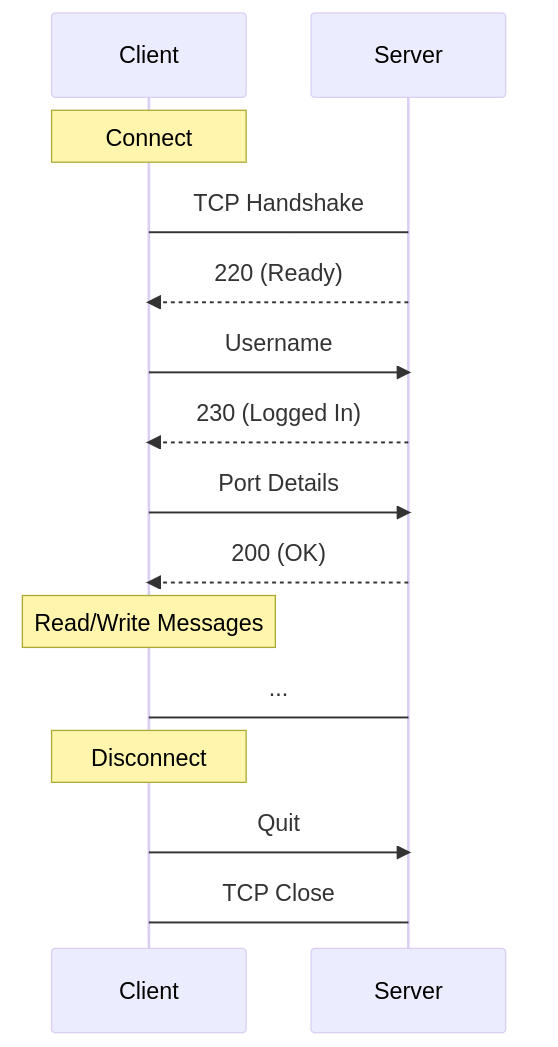
\includegraphics[width=0.6\linewidth]{ftp-conn-sequence.png}
    \caption{FTP Connection Sequence}
    \label{fig:ftp-conn-sequence}
\end{figure}

\begin{figure}[h!]
    \centering
    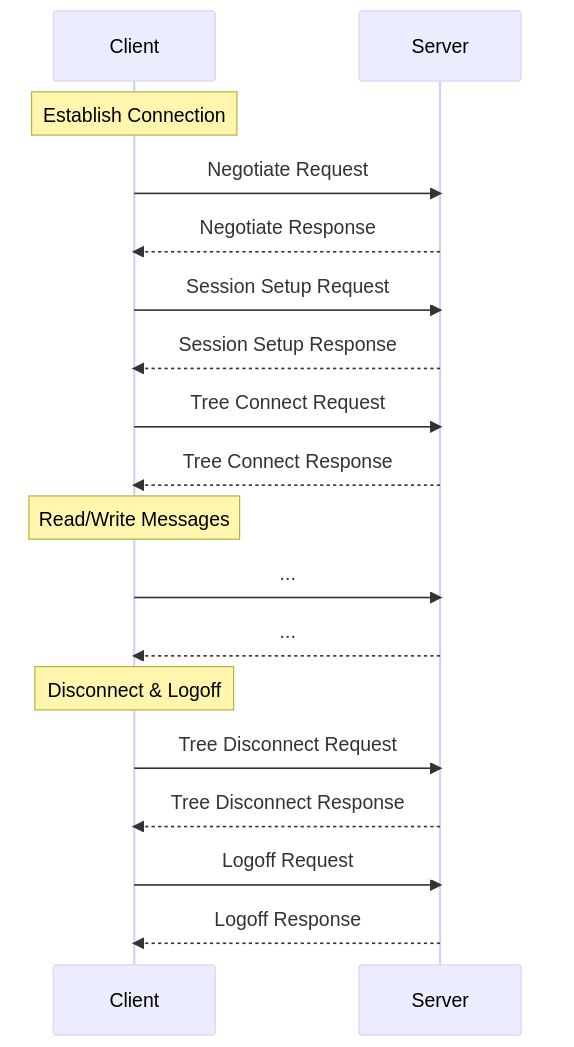
\includegraphics[width=0.6\linewidth]{smb2-conn-sequence.png}
    \caption{SMB2 Connection Sequence}
    \label{fig:smb2-conn-sequence}
\end{figure}

\chapter{Links}
\begin{itemize}
    \label{project-links}
    \item Project Repository: \url{https://github.com/enchant97/file-sync-protocol}
    \item Testing Configuration: \url{https://github.com/enchant97/file-sync-protocol/tree/main/scripts/test-servers}
    \item Prototype One: \url{https://github.com/enchant97/file-sync-protocol/tree/main/prototypes/proto-1}
    \item Prototype Two: \url{https://github.com/enchant97/file-sync-protocol/tree/main/prototypes/proto-2b}
    \item Prototype Three: \url{https://github.com/enchant97/file-sync-protocol/tree/main/prototypes/proto-3}
\end{itemize}


\glsaddallunused
\end{document}
